% Goals 

\section{C\# Grundlagen}
Ähnlichkeiten zu Java: Objektorientierung, Interfaces, Exceptions, Threads, Namespaces (wie Packages), Strenge Typenprüfung, Garbage Collection, Reflection un d dynamisches Laden von Code.
Neues: Referenzparameter, Objekte am Stack, Blockmatrizen, Enumerationstypen, Uniformes Typensystem, goto, Systemnahes Programmieren, Versionierung.

\subsection{Naming Guidelines}
\begin{figure}[h!]
	\centering
  	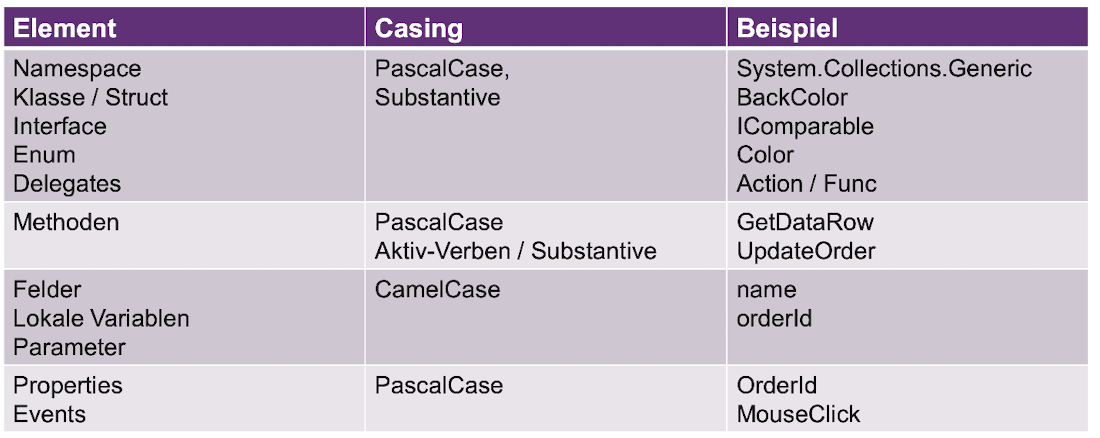
\includegraphics[width=0.75\textwidth]{namingguide}
    \caption{Naming Guidelines}
\end{figure}

\subsection{Sichtabrkeitsattribute}
\begin{figure}[h!]
	\centering
  	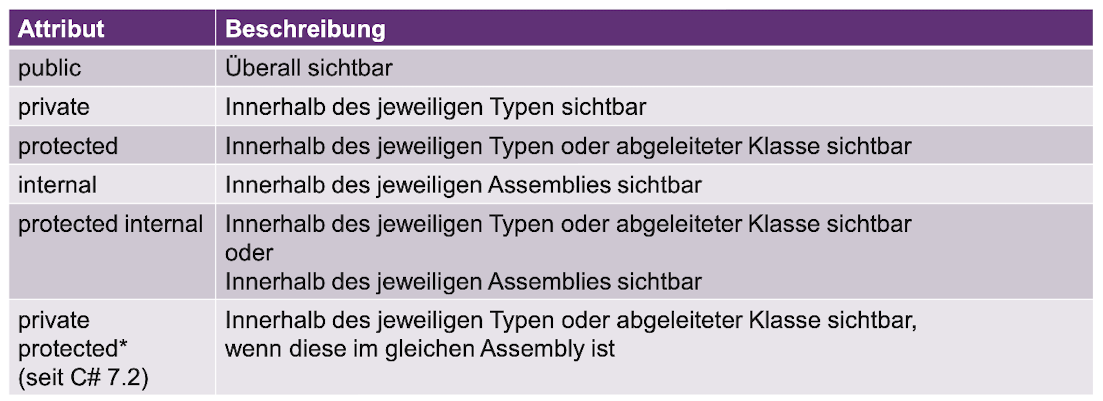
\includegraphics[width=0.75\textwidth]{sichtbarkeitsattribute}
    \caption{Sichtabrkeitsattribute}
\end{figure}

\begin{figure}[h!]
	\centering
  	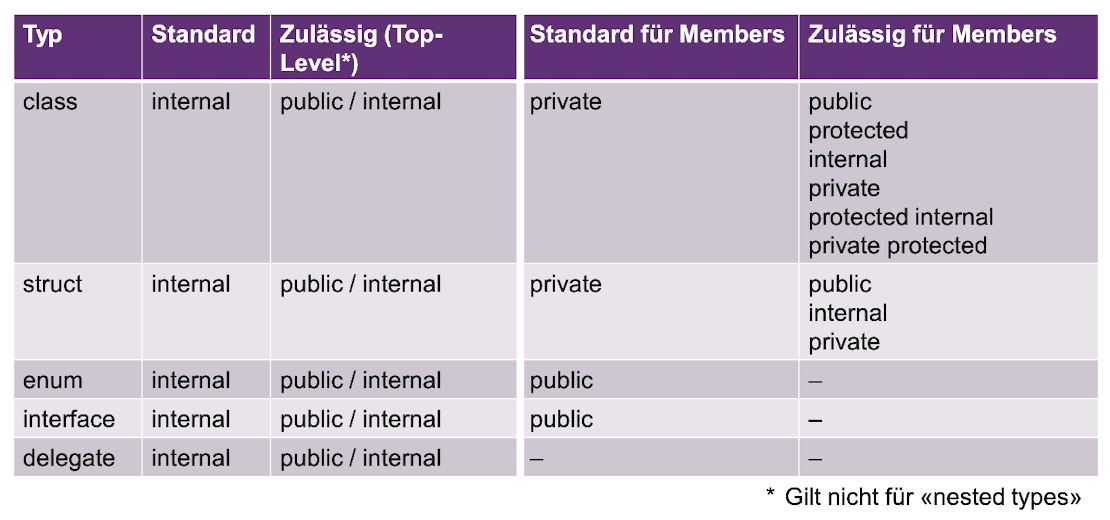
\includegraphics[width=0.75\textwidth]{sichtbarkeit}
    \caption{Standard Sichtbarkeiten von Typen}
\end{figure}

\subsection{Primitivtypen}
\textbf{Ganzzahlen}\\
Numerisch Werte können für eine bessere Lesbarkeit mit dem "\_" geschrieben werden.
Bestimmung des Typen: Ohne Suffix=kleinster Type aus int, uint, long, ulong. Suffix u | U =kleinster Type aus uint, ulong. Suffix l | L = kleinster Type aus long, ulong.

\textbf{Fliesskommazahlen}\\
Bestimmung des Typen: Ohne Suffix=double. Suffix f | F=float. Suffix d | D=double. Suffix m | M=decimal.

\textbf{Typenkompatibilität}
\begin{figure}[h!]
	\centering
  	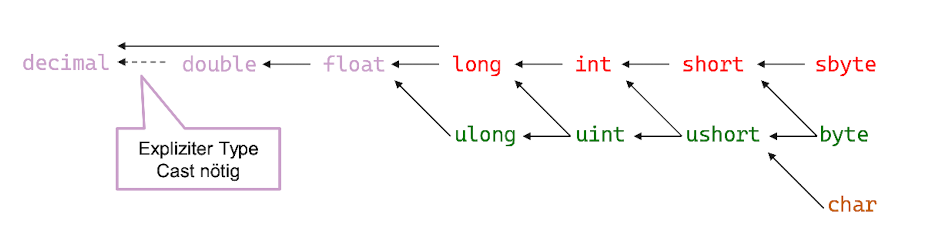
\includegraphics[width=0.75\textwidth]{typecast}
    \caption{Typenkompatibilität}
\end{figure}

\subsection{Statements}
\begin{minipage}[]{0,5\linewidth}
\textbf{If Statements}
\begin{lstlisting}
int value = 5;
if (0 >= value && value < 9) {
	/* ... */
} else if (value > 10) {
	/* ... */
} else {
	Console.WriteLine("Invalid: " + value);
}
\end{lstlisting}
\textbf{Switch Statement} 
\begin{lstlisting}
string ctry = "Germany"; string language; 
switch (ctry) {
	case "England": 
	case "USA":
		language = "English"; break;
	case "Germany": 
	case "Austria": 
	case "Switzerland":
		language = "German"; break;
	case null:
		Console.WriteLine("Coutry null"); break;
	default:
		Console.WriteLine("Unknown" + ctry); break;
}
\end{lstlisting} 
\end{minipage}
\begin{minipage}{0,5\linewidth}
\textbf{Loops}
\begin{lstlisting}
// Kopfgesteuert
int i = 1;
int sum = 0;
while (i <= 3)
{
	sum += i; 
	i++;
}
// Fussgesteuert
int i = 1;
int sum = 0;
do
{
	sum += i; 
	i++;
} while (i <= 3)	
// Foreach
int[] a = { 3, 17, 4, 8, 2, 29 };
foreach (int x in a)
{
	sum += x;
}
\end{lstlisting}
\textbf{Jumps}
\begin{lstlisting}
for (int i = 0; i < 10; i++) {
	if (i == 1) { continue; } 
	if (i == 3) { goto myLabel; } 
	if (i == 5) { break; }
Console.WriteLine(i);
myLabel: ; 
}
\end{lstlisting} 
\end{minipage}

\subsection{Namespaces}
Entspricht in Java dem Package. Strukturiert den Quellcode und ist hierarchisch aufgebaut. Beinhaltet: Andere Namespaces, Klassen, Interfaces, Structs, Enums, Delegates.

\subsection{Main Methode}
Einstiegspunkt (entry point) eines Programmes. Zwingend nötig für Executables (Console Application, Windows Application etc.) Klassischerweise genau 1x mal erlaubt. Wenn mehrere Main-Methoden vorhanden sind, muss dies in der Projektdatei angegeben werden.

\subsubsection{Top-Level Satements}
Erlaubt das Weglassen der Main-Methode als entry point. Vereinfacht z.B. Beispiel-Applikationen. \\
\textbf{Regeln:}
\begin{itemize}
  \itemsep -0.5em 
  \item Nur 1x pro Assemlby erlaubt
  \item Arugmente heissen fix args
  \item Exit Codes erlaubt
  \item VOR dem top-level statements können usings definiert werden.
  \item NACH dem top-level satements können Typen definiert werden.
\end{itemize}

\begin{lstlisting}
using System;
for (int i = 0; i < args.Length; i++) {
	ConsoleWriter.Write(args, i);
{
Class ConsoleWriter {
	public static void Write(string[] args, in t) // Top Level Satement
	{
		Console.WriteLine("Arg {i} O {args[i]}");
	}
}
\end{lstlisting}

\subsection{Enumerationstypen}
Ist eine Liste vordefinierter Konstanten inklusive Wert (Default-Typ Int32). Der erste Wert ist per defualt eine 0 und die andere folgen n+1.
\begin{lstlisting}
enum Days { Monday, Tuesday, Wednesday, Thursday, Friday, Saturday };
Days today = Days.Monday;
if (today == Days.Monday) { /* ... */ }
enum Days { Monday = 10, Tuesday, Wednesday, Thursday, Friday, Saturday };
enum Days:byte { Sunday, Monday, Tuesday, Wednesday, Thursday, Friday, Saturday };
// Parsing
bool success3 = Enum.TryParse("Monday", out Days day3);
\end{lstlisting}

\subsection{Object}
System.Object ist die Basisklasse für alle Typen und Objekte. Das keyword object is ein Alias für System.Object. 

\begin{lstlisting}
o1 = "Test";	o1 = 123;	o1 = new Rectangle();
void Push(object x) { /* ... */ }
Push("Test"); Push(123);
Push(new Rectangle());
Push(new int[3]);
\end{lstlisting}

\subsection{Arays}
Einfachste Datenstruktur für Listen, Ausprägungen: Eindimensional, Mehrdimensional (Rechteckig), Mehrdimensional Jagged (Ausgefranst). Länge aller Dimensinen müssen bei der Instanzierung bekannt sein. Alle Werte sind nach der Instanzierung initialisiert (false, 0, null etc.). Arrays sind eine Klasse und leben immer auf dem Heap!

\begin{lstlisting}
// Eindimensionale Arrays
int[] array1 = new int[5];                   // Deklaration (Value Type)
int[] array2 = new int[] { 1, 3, 5, 7, 9 };  // Deklaration & Wertdefinition
int[] array3 = int[] { 1, 2, 3, 4, 5, 6 };   // Vereinfachte Syntax ohne new
int[] array4 = { 1, 2, 3, 4, 5, 6 };     // Vereinfachte Syntax ohne new Typ
object[] array5 = new object[5];             // Deklaration (Reference Type)
// Mehrdimensionale Arrays
int[,] multiDim1 = new int[2, 3];                 // Deklaration
int[,] multiDim2 = { { 1, 2, 3 }, { 4, 5, 6 } };  // Deklaration&Wertdefinition
// Mehrdimensionale Arrays Jagged
int[][] jaggedArray = new int[6][];          // Deklaration
jaggedArray[0] = new int[] { 1, 2, 3, 4 };   // Wertdefinition
\end{lstlisting}

\subsection{Strings}
Datenstruktur für Zeichenketten. Eigenschaften: Reference Type, string ist Alias für "System.String", nicht modifizierbar, Verkettung möglich, Wertevergelich mit == oder Equals Methode möglich. Nicht Null/0 terminiert, Indexierung möglich, Länge wird durch das Property "Length" ermittelt.\\
\textbf{Interning} \\
Strings werden intern wiederverwendet und ein gleicher String nicht unbedingt kopiert. Erst "string.Copy(...) erzeugt eine echte Kopie.
\begin{lstlisting}
string s1 = "Hello ";
string s2 = "World";
string s3 = s1 + s2;
// Unveraenderbarkeit wird durch den Compiler sichergesetllt
string s1 = "Hello ";
string s2 = "World";
string s3 = s1 + s2; // string s3 = System.String.Concat(s1, s2); 
s3 += "!";           // s3 = System.String.Concat(s3, "!"); 
// String Interpolation
string s3 = $"{DateTime.Now}: {"Hello"}";
string s4 = $"{DateTime.Now}: {(DateTime.Now.Hour < 18 ? "Hello" : "Good Evening")}";
\end{lstlisting}

\subsection{Symbole}
Sind Unicode codiert und Case-Sensitive. @ für Verwendung von Schlüsselwörtern als Identifier. 


\pagebreak



